\section{Evaluation}
\label{sec:eval}

\subsection{Experimental Setup}
\label{sec:eval:setup}

\paragraph{Platforms.}

We evaluate six GPU platforms. The four discrete GPUs are NVIDIA A100,
RTX~4090, RTX~3080, and RTX~4070 Laptop. The embedded platforms are Jetson
Xavier NX and AGX Orin; we also measure board energy on both. The discrete
platforms use PyTorch 2.1.2, CUDA 12.1, and cuDNN 8.9.2; both Jetson platforms
use PyTorch 2.1.0, CUDA 11.4, and cuDNN 8.6. All paths in the full workload
comparison use FP32 (SIMT) with TF32 disabled. Sensitivity studies additionally
evaluate FP16 (tensor core) on selected platforms. On each platform, all backends run under the same fixed clock and
power configuration.

\paragraph{Models, tasks, and mask sources.}
Our workloads (Table~\ref{tab:models}) span three vision tasks:
FireFlowNet~\cite{fireflownet} for event-based optical flow on
MVSEC~\cite{mvsec} with Ev-Conv~\cite{evconv} masks,
YOLOv8n and YOLOv8m~\cite{yolov8} for detection on MOT16~\cite{mot16} with
DeltaCNN's~\cite{deltacnn} temporal masks, and
DynConv~\cite{dynconv} for human pose on MPII~\cite{mpii} with learned spatial
gates. For every workload, calibration uses the training split, while all
reported results use a disjoint test split with the authors' released
weights~\cite{fireflownet,yolov8,dynconv}. Within each workload, we fix
inputs, weights, and upstream mask policy; every sparse path receives the same
layer masks, isolating the masked-convolution backend.

\begin{table}[htb]
\centering
\caption{Evaluation workloads.}
\label{tab:models}
\footnotesize
\setlength{\tabcolsep}{3pt}
\renewcommand{\arraystretch}{1.08}
\begin{tabular}{@{}
  >{\raggedright\arraybackslash}p{0.19\columnwidth}
  >{\centering\arraybackslash}p{0.22\columnwidth}
  >{\centering\arraybackslash}p{0.22\columnwidth}
  >{\centering\arraybackslash}p{0.22\columnwidth}@{}}
\hline
 & \textbf{FireFlowNet} \cite{fireflownet}
 & \textbf{YOLOv8n/m} \cite{yolov8}
 & \textbf{DynConv} \cite{dynconv} \\
\hline
Task & Optical flow & Detection & Human pose \\
Mask source & Ev-Conv~\cite{evconv} & DeltaCNN~\cite{deltacnn}
            & DynConv~\cite{dynconv} \\
Dataset & MVSEC~\cite{mvsec} & MOT16~\cite{mot16} & MPII~\cite{mpii} \\
Input size & $256{\times}256$ & $640{\times}640$ & $256{\times}256$ \\
Parameters & 0.056M & 3.16M~/~25.9M & 6.89M \\
Eval. samples & 196.8K & 2,575 & 2,958 \\
\hline
\end{tabular}
\end{table}

\paragraph{Baselines.}
We compare \sysname against three FP32 (SIMT) execution paths:
\textbf{Dense} (PyTorch/cuDNN~\cite{cudnn} with autotuning),
\textbf{Tile skipping} (DeltaCNN~\cite{deltacnn} for FireFlowNet and YOLO;
DynConv supplies output masks directly), and
\textbf{Gather-scatter} (DynConv's~\cite{dynconv} CUDA backend for pose;
MMCV's~\cite{mmcv} MaskedConv2d for FireFlowNet and YOLO).

\paragraph{Measurements.}

We measure per-frame full-model GPU latency over the complete evaluation
datasets. CUDA events bracket each frame's inference; after warm-up we run
three complete rounds and average per-frame latency across all frames and
rounds. The interval includes mask propagation, worklist construction, all
network operators, and output update; it excludes input transfer, offline
calibration, and one-time initialization. We report $\eta$, $T$, and
$T_{\mathrm{eff}}$ at the model level by accumulating required and issued
work across layers per frame (Eq.~\ref{eq:efficiency-framework}), then
averaging across frames. On the Jetson platforms, we integrate board-level
\texttt{VDD\_IN} power over each frame interval to obtain per-frame energy.
For accuracy, we follow the original protocols: AEE for optical
flow~\cite{evconv}, AP for detection~\cite{deltacnn}, and PCKh for
pose~\cite{dynconv}. MOT16 AP uses fixed pseudo-labels from a dense YOLO26x
teacher~\cite{yolo26} because ground-truth detections cover only the training
split.

\subsection{End-to-End Performance}
\label{sec:eval:end-to-end}

\begin{figure*}[htb]
  \centering
  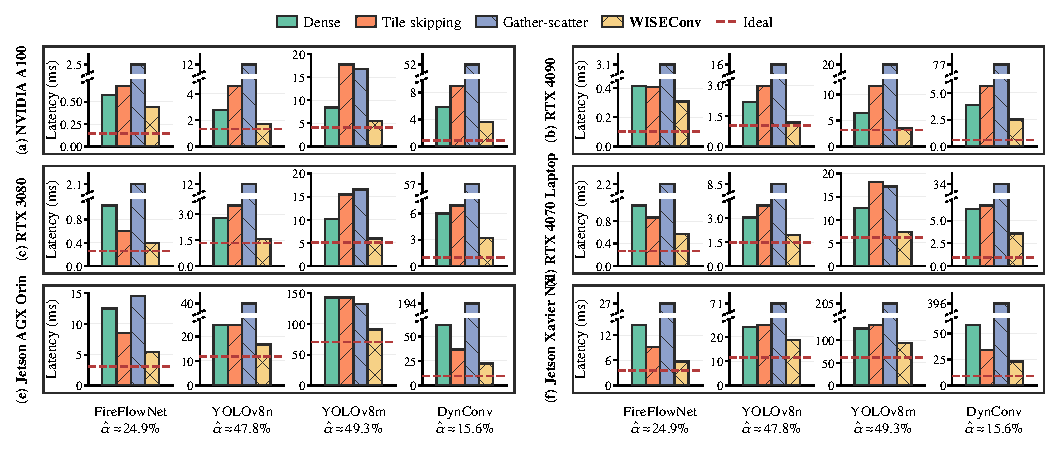
\includegraphics[width=\textwidth]{figures/e2e_latency.pdf}
  \caption{Full-model mean per-frame latency across GPU platforms. Each
  workload uses an independent y-axis. Labels report the model-level active
  ratio $\hat{\alpha}$, aggregated as described in
  \S\ref{sec:eval:setup} and averaged across evaluation sequences. Red dashed
  lines mark ideal proportional scaling, computed by applying each sequence's
  model-level active ratio to its dense latency before aggregation.}
  \Description{Grouped bar charts of full-model latency. Six platform panels
  each contain four workload groups comparing Dense, Tile skipping,
  Gather-scatter, and WISEConv. Selected workload groups use broken y-axes for
  a much slower gather-scatter path. Red dashed lines show the ideal
  proportional-scaling reference for each workload and platform, and workload
  labels report their aggregated active ratios.}
  \label{fig:e2e-latency}
\end{figure*}

\paragraph{Latency.}
\sysname is the fastest path in all 24
measured workload-platform pairs (Figure~\ref{fig:e2e-latency}). Relative to
the fastest evaluated competing path in each pair, it achieves a 1.57$\times$
geometric-mean speedup; individual-pair speedups range from 1.28$\times$ to
1.87$\times$, corresponding to 22.1--46.5\% lower latency. These gains persist
despite a more than two-order-of-magnitude span in absolute latency, from
0.309\,ms for FireFlowNet on RTX~4090 to 94.3\,ms for YOLOv8m on Xavier NX.

Unlike existing sparse paths, \sysname delivers uniform gains across workload
regimes. Dense is the fastest evaluated competing path in 15 of the 24
pairs, compared with eight for tile skipping and only one for gather-scatter;
sparsity magnitude alone does not determine where an existing sparse path
crosses the dense baseline.

\sysname's lead over the per-pair fastest competing path is narrower on the
embedded platforms (geometric mean 1.48$\times$ on Jetson vs.\ 1.62$\times$ on
discrete GPUs), though it remains fastest in all eight Jetson pairs, because
sparse paths are more effective on the narrower Jetson GPUs, leaving less
headroom.

\sysname also realizes more of the available sparsity headroom than every
competing path, running at 1.09--4.18$\times$ the ideal proportional-scaling
reference while the fastest competing path remains at 1.88--6.43$\times$.

\paragraph{Energy.}
\sysname is the lowest-energy path for every workload on both Jetson
platforms (Table~\ref{tab:e2e-energy}), reducing energy by
17.0--39.8\% relative to the lowest-energy competing path in each pair and by
28.5--72.6\% relative to dense execution.

% Generated by figures/plot_e2e.py from figures/e2e_stats.csv.
\begin{table}[b]
  \centering
  \caption{Per-frame board energy (J) on the Jetson platforms. Parentheses report each sparse path's change relative to Dense.}
  \label{tab:e2e-energy}
  \footnotesize
  \setlength{\tabcolsep}{1.2pt}
  \renewcommand{\arraystretch}{1.08}
  \begin{tabular}{@{}cc@{\hspace{4.0pt}}cccc@{}}
    \toprule
    \begin{tabular}[c]{@{}c@{}}GPU\end{tabular} & \begin{tabular}[c]{@{}c@{}}System\end{tabular} & \begin{tabular}[c]{@{}c@{}}FireFlowNet\end{tabular} & \begin{tabular}[c]{@{}c@{}}YOLOv8n\end{tabular} & \begin{tabular}[c]{@{}c@{}}YOLOv8m\end{tabular} & \begin{tabular}[c]{@{}c@{}}DynConv\end{tabular} \\
    \midrule
    \multirow{4}{*}{\rotatebox[origin=c]{90}{AGX Orin}} & Dense & 0.26 & 0.48 & 2.70 & 1.20 \\
     & Tile skip & 0.15\,(-43.8\%) & 0.44\,(-9.1\%) & 2.33\,(-13.7\%) & 0.67\,(-44.7\%) \\
     & Gather & 0.29\,(+9.5\%) & 0.70\,(+46.1\%) & 2.42\,(-10.4\%) & 2.37\,(+97.0\%) \\
     & \textbf{WISEConv} & \textbf{0.10}\,(-61.6\%) & \textbf{0.32}\,(-33.9\%) & \textbf{1.57}\,(-41.7\%) & \textbf{0.48}\,(-60.4\%) \\
    \midrule
    \multirow{4}{*}{\rotatebox[origin=c]{90}{Xavier NX}} & Dense & 0.28 & 0.49 & 2.58 & 1.08 \\
     & Tile skip & 0.13\,(-54.5\%) & 0.42\,(-13.8\%) & 2.27\,(-12.2\%) & 0.54\,(-50.4\%) \\
     & Gather & 0.33\,(+17.0\%) & 0.85\,(+75.8\%) & 3.18\,(+23.2\%) & 2.83\,(+160.9\%) \\
     & \textbf{WISEConv} & \textbf{0.08}\,(-72.6\%) & \textbf{0.35}\,(-28.5\%) & \textbf{1.78}\,(-31.1\%) & \textbf{0.34}\,(-68.5\%) \\
    \bottomrule
  \end{tabular}
\end{table}


\paragraph{Accuracy.}
\begin{figure}[htb]
  \centering
  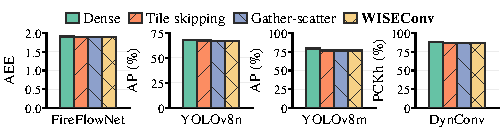
\includegraphics[width=\columnwidth]{figures/e2e_accuracy.pdf}
  \caption{Task accuracy on RTX~3080 under the evaluated upstream sparsity
  policies, measured by AEE~($\downarrow$), AP~($\uparrow$), and
  PCKh~($\uparrow$).}
  \Description{Four grouped bar charts compare Dense, Tile skipping,
  Gather-scatter, and WISEConv task accuracy. FireFlowNet reports average
  endpoint error, YOLOv8n and YOLOv8m report AP, and DynConv reports
  PCKh. The three sparse execution paths have closely matching task accuracy in
  every workload.}
  \label{fig:e2e-accuracy}
\end{figure}
\sysname's latency and energy gains do not alter accuracy:
AEE and PCKh match the other sparse paths at the reported precision, and
YOLOv8 AP differs by at most 0.5\% (Figure~\ref{fig:e2e-accuracy}).


\subsection{Microbenchmarks}
\label{sec:eval:microbenchmarks}

\begin{table}[!t]
  \centering
  \caption{WISEConv $\eta$ decomposition and worklist-length statistics
  on RTX~3080. The $n_{\mathcal{W}}$ percentiles are computed from worklist
  lengths pooled across all layers and frames.}
  \Description{A table reports eta construct, eta compute, eta, and the
  P10, P50, and P90 worklist lengths for FireFlowNet, YOLOv8n, YOLOv8m,
  and DynConv on RTX 3080. Worklist-length statistics are computed from samples
  pooled across all layers and frames.}
  \label{tab:worklist-efficiency}
  \footnotesize
  \setlength{\tabcolsep}{1.5pt}
  \renewcommand{\arraystretch}{1.12}
  \begin{tabular*}{\columnwidth}{@{\extracolsep{\fill}}l c c c r r r@{}}
    \hline
    \multirow{2}{*}{\textbf{Workload}} &
    \multirow{2}{*}{$\boldsymbol{\eta}_{\mathrm{construct}}$} &
    \multirow{2}{*}{$\boldsymbol{\eta}_{\mathrm{compute}}$} &
    \multirow{2}{*}{$\boldsymbol{\eta}$} &
    \multicolumn{3}{c}{$\boldsymbol{n}_{\mathcal{W}}$} \\
    \cline{5-7}
    & & & & \textbf{P10} & \textbf{P50} & \textbf{P90} \\
    \hline
    FireFlowNet & 99.9\% & 99.1\% & 98.9\% & $1{,}303$ & $15{,}083$ & $33{,}880$ \\
    YOLOv8n & 98.5\% & 97.7\% & 96.2\% & $77$ & $937$ & $5{,}937$ \\
    YOLOv8m & 98.7\% & 96.5\% & 95.2\% & $75$ & $840$ & $6{,}110$ \\
    DynConv & 100.0\% & 81.7\% & 81.7\% & $3$ & $43$ & $389$ \\
    \hline
  \end{tabular*}
\end{table}


\paragraph{Effective throughput.}
Under the same settings, we estimate
full-model throughput $T$ and effective throughput $\eta T$ on RTX~3080 and
AGX Orin (Figure~\ref{fig:effective-throughput}). \sysname sustains


30.7--87.2\% of Dense raw throughput on RTX~3080 and 58.6--83.5\% on AGX
Orin, the highest raw throughput among the sparse paths in every workload.
DeltaCNN's lower raw throughput reflects the impact of routing very sparse
tiles through its fused selective path~\cite{deltacnn}. The two YOLO workloads
lie at the upper end because their higher active ratios expose more parallelism
and amortize fixed costs. Combining throughput and useful-compute ratio,
\sysname reaches 1.52--1.78$\times$ the strongest competing effective
throughput on RTX~3080 and 1.45--1.65$\times$ on AGX Orin.

Table~\ref{tab:worklist-efficiency} localizes the remaining wasted work on
RTX~3080. Its $\eta_{\mathrm{construct}}$ stays at 98.5--100.0\%, while the
selected decompositions give $\eta_{\mathrm{compute}}=96.7$--$99.1\%$ for
FireFlowNet and the two YOLO workloads. DynConv instead has
$\eta_{\mathrm{compute}}=90.1\%$: its low
active ratio and small spatial grids yield exceptionally short worklists
(P10, P50, and P90 lengths of 3, 43, and 389), making final-tile padding
proportionally large. Because its inputs are temporally unrelated, DynConv uses
the same exact-length device policy without a temporal activity selector. Even
in this setting, this ratio
is substantially above tile skipping's 48.9\% on RTX~3080.
\begin{figure}[h]
  \centering
  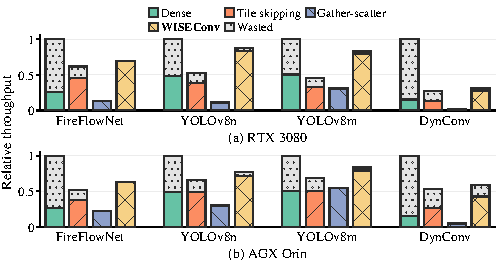
\includegraphics[width=\columnwidth]{figures/effective_throughput.pdf}
  \caption{Full-model effective throughput $\eta T$ and wasted throughput
  $(1-\eta)T$ on RTX~3080 and AGX Orin, normalized within each platform to
  Dense raw throughput.}
  \Description{Two vertically stacked platform panels compare Dense, Tile
  skipping, Gather-scatter, and WISEConv across four workloads. Each bar is
  divided into effective and wasted throughput, normalized to Dense raw
  throughput on the same platform.}
  \label{fig:effective-throughput}
\end{figure}

\begin{table}[!ht]
  \centering
  \caption{Full-model YOLOv8n cost decomposition in time (ms) and
  percentage on RTX~3080. Cost is classified into worklist construction
  (Cons.), convolution (Conv.), elementwise operators (Elem.), and other
  cost.}
  \Description{A table divides every YOLOv8n frame into low- and
  high-activity halves and compares full-model latency attributed to
  construction, convolution, elementwise, and other work for Dense, Tile
  skipping, Gather-scatter, and WISEConv. Construction is applicable only
  to WISEConv.}
  \label{tab:cost-decomposition}
  \footnotesize
  \setlength{\tabcolsep}{1.2pt}
  \renewcommand{\arraystretch}{1.15}
  \begin{tabular}{@{}c c c c c c c@{}}
    \hline
      & \textbf{System} & \textbf{Tot.} & \textbf{Cons.} &
      \textbf{Conv.} & \textbf{Elem.} & \textbf{Other} \\
    \hline
    \multirow{4}{*}{\rotatebox[origin=c]{90}{Low (40.7\%)}} & Dense & 2.79 & \textemdash{} & 2.54(91.2\%) & 0.14(5.0\%) & 0.10(3.7\%) \\
    & Tile skipping & 3.42 & \textemdash{} & 3.09(90.3\%) & 0.16(4.6\%) & 0.17(5.1\%) \\
    & Gather & 11.81 & \textemdash{} & 0.73(6.2\%) & 0.09(0.7\%) & 11.00(93.1\%) \\
    & \textbf{WISEConv} & 1.47 & 0.10(7.1\%) & 1.09(73.8\%) & 0.12(8.2\%) & 0.16(10.9\%) \\
    \hline
    \multirow{4}{*}{\rotatebox[origin=c]{90}{High (56.7\%)}} & Dense & 2.79 & \textemdash{} & 2.54(91.2\%) & 0.14(5.0\%) & 0.10(3.7\%) \\
    & Tile skipping & 3.59 & \textemdash{} & 3.25(90.4\%) & 0.17(4.7\%) & 0.18(4.9\%) \\
    & Gather & 11.82 & \textemdash{} & 0.83(7.0\%) & 0.09(0.8\%) & 10.90(92.2\%) \\
    & \textbf{WISEConv} & 1.69 & 0.11(6.2\%) & 1.29(76.3\%) & 0.13(7.7\%) & 0.17(9.8\%) \\
    \hline
  \end{tabular}
  \par\vspace{6pt}
  \noindent\parbox{\columnwidth}{\footnotesize\textit{Notes.} Low and High split
  all frames from the evaluated MOT16 test sequences at the median
  per-frame active ratio; their parenthesized labels report bin means.
  We obtain each stage time by multiplying its per-frame NSYS fraction
  by the corresponding CUDA-event latency from the end-to-end
  evaluation.}
\end{table}


\paragraph{Latency cost decomposition.}
We decompose full-model YOLOv8n latency by execution stage on RTX~3080 and AGX
Orin (Table~\ref{tab:cost-decomposition}). On the randomly sampled RTX~3080
frames, \sysname reduces the convolution share from 2.55 to 1.10\,ms while
adding only 0.10\,ms of construction; the corresponding sampled-row totals
are 2.79 and 1.49\,ms. On AGX Orin, construction accounts for 0.37\,ms, while convolution falls
from 22.61 to 13.41\,ms and the total falls from 25.09 to
17.07\,ms.

Gather-scatter has the lowest convolution time but \emph{Other} (extraction,
scatter, GEMM setup) accounts for 92\% of its total on RTX~3080, showing that
exact selection alone is insufficient without direct worklist consumption.

% Optional CUDA-level diagnostics are not a third required microbenchmark.
% If the two figures leave a concrete locality question, the useful diagnostic
% is whether tile-local worklists preserve dense-like cache behavior on the
% same real frames: collect L2 hit rate together with L2/DRAM traffic per
% required FLOP for Dense, WISEConv, and a sparse comparator.  L2 hit rate alone
% is insufficient because a path may issue fewer requests or transfer more
% bytes per useful output; report it only with traffic and the measured
% throughput, and keep the result as a small diagnostic rather than a
% standalone counter survey.

\paragraph{Memory overhead.}
Table~\ref{tab:memory} reports peak GPU memory. \sysname uses 10--12\% more
memory than tile skipping on the YOLO workloads, due to worklist buffers and
the partial-reduction workspace $\mathbf{Z}$; FireFlowNet's overhead is larger
(39\%) because its small model amplifies the fixed buffer cost. DynConv's gather-scatter backend reports the lowest footprint
because many of its layers do not maintain dense-layout intermediate tensors.

\begin{table}[htb]
  \centering
  \caption{Peak GPU memory (MiB) on RTX~3080.}
  \label{tab:memory}
  \footnotesize
  \setlength{\tabcolsep}{4pt}
  \renewcommand{\arraystretch}{1.08}
  \begin{tabular}{@{}lrrrr@{}}
    \hline
    \textbf{Workload} & \textbf{Dense} & \textbf{Tile skip} & \textbf{Gather-scatter} & \textbf{\sysname} \\
    \hline
    FireFlowNet & 65.9 & 174.1 & 166.0 & 242.1 \\
    YOLOv8n     & 164.9 & 253.2 & 238.7 & 279.7 \\
    YOLOv8m     & 195.1 & 854.3 & 825.7 & 956.2 \\
    DynConv     & 83.7 & 80.9 & 27.1 & 99.1 \\
    \hline
  \end{tabular}
\end{table}

\subsection{Ablation Study and Sensitivity Analysis}
\label{sec:eval:ablation-sensitivity}

\begin{table}[htb]
  \centering
  \caption{YOLOv8n component ablation on RTX~3080 and AGX~Orin.
  Times are milliseconds.}
  \Description{A table compares seven WISEConv design variants on RTX
  3080 and AGX Orin. Each platform reports useful-compute ratio,
  construction time, convolution time, and full-model latency.}
  \label{tab:ablation}
  \fontsize{7.0}{7.8}\selectfont
  \setlength{\tabcolsep}{0.7pt}
  \renewcommand{\arraystretch}{1.06}
  \begin{tabular*}{\columnwidth}{@{\extracolsep{\fill}}l c r r r c r r r@{}}
    \hline
    \multirow{2}{*}{\textbf{Variant}} &
    \multicolumn{4}{c}{\textbf{RTX 3080}} &
    \multicolumn{4}{c}{\textbf{AGX Orin}} \\
    \cline{2-5}\cline{6-9}
    & $\boldsymbol{\eta}$ & \textbf{Cons.} & \textbf{Conv.} & \textbf{Total}
    & $\boldsymbol{\eta}$ & \textbf{Cons.} & \textbf{Conv.} & \textbf{Total} \\
    \hline
    Atomic append   & 95.6\% & 0.169 & 1.241 & 1.862 & 93.1\% & 0.538 & 12.984 & 17.065 \\
    Global order    & 95.6\% & 0.265 & 1.180 & 1.897 & 93.1\% & 0.695 & 12.894 & 17.426 \\
    No reuse        & 97.0\% & 0.226 & 1.184 & 1.862 & 94.5\% & 0.648 & 12.739 & 17.112 \\
    DP only         & 95.5\% & 0.113 & 1.561 & 2.127 & 93.1\% & 0.359 & 13.940 & 17.942 \\
    No Hybrid       & 95.5\% & 0.113 & 1.227 & 1.793 & 93.1\% & 0.359 & 13.189 & 17.191 \\
    Sync exact selector & 95.5\% & 0.113 & 0.945 & 6.695 & 93.8\% & 0.352 & 10.328 & 23.787 \\
    \textbf{Ours}   & 95.5\% & 0.113 & 1.189 & 1.754 & 93.1\% & 0.359 & 12.994 & 16.996 \\
    \hline
  \end{tabular*}
\end{table}


Table~\ref{tab:ablation} isolates the construction and consumption choices on
YOLOv8n. On RTX~3080, Ours achieves 95.5\% useful-compute ratio at
1.754\,ms. Atomic append, Global order, and No reuse raise latency by
6.2\%, 8.2\%, and 6.2\%, respectively, exposing the cost of global
coordination and per-layer reconstruction. DP only is
21.3\% slower, whereas No Hybrid adds only 2.2\%.
Synchronizing the exact worklist length to the host costs 6.695\,ms
(3.82$\times$ Ours), confirming that host readback dominates any gain from
exact launch sizing.
On AGX~Orin the construction variants show smaller margins (0.4--2.5\%)
because convolution dominates the total. DP only adds 5.6\% and
Sync exact selector reaches 23.787\,ms (1.40$\times$): although its
convolution is faster (the host-selected tile count enables a tighter
decomposition), the per-operator synchronization adds 6.8\,ms of overhead
that erases the gain.

\begin{figure}[htb]
  \centering
  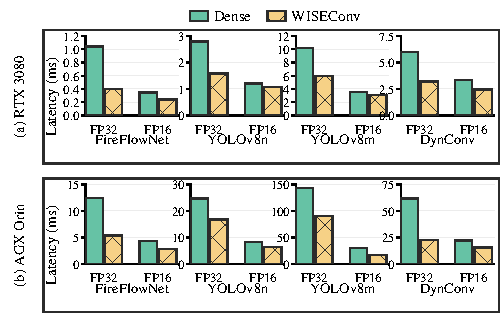
\includegraphics[width=\columnwidth]{figures/dtype_sensitivity.pdf}
  \caption{FP32 (SIMT) vs.\ FP16 (tensor core) full-model latency for
  Dense and \sysname across all four workloads. FP16 \sysname values for
  YOLOv8n and YOLOv8m are estimates from per-layer profiling.}
  \Description{Two panels (RTX 3080 and AGX Orin) each show four workload
  groups comparing Dense and WISEConv in FP32 and FP16.}
  \label{fig:dtype-sensitivity}
\end{figure}

\paragraph{Tensor core sensitivity.}
Figure~\ref{fig:dtype-sensitivity} compares FP32 and FP16 execution on
RTX~3080 and AGX~Orin. \sysname retains an end-to-end gain under tensor cores
on both platforms across all four workloads, although the gain narrows relative
to FP32 because tensor cores reduce the convolution time that \sysname saves
by skipping, shrinking the absolute saving while non-convolution costs
(construction, elementwise, mask processing) remain unchanged.

\begin{table}[!ht]
  \centering
  \caption{Stream-level batch sensitivity for full-model YOLOv8n on
  RTX~3080, decomposed by execution stage. All times are amortized
  ms/frame; parentheses report each stage's share of total latency.}
  \Description{A table compares Dense, Tile skipping, Gather-scatter,
  and WISEConv at batch sizes one, four, and eight. Each row gives
  amortized total latency per frame and its division among worklist
  construction, convolution, elementwise, and other work.}
  \label{tab:batch-cost-decomposition}
  \footnotesize
  \setlength{\tabcolsep}{1.0pt}
  \renewcommand{\arraystretch}{1.10}
  \begin{tabular}{@{}c@{\hspace{2pt}}l r c c c c@{}}
    \hline
    \textbf{B} & \textbf{System} & \textbf{Tot.} & \textbf{Cons.} &
    \textbf{Conv.} & \textbf{Elem.} & \textbf{Other} \\
    \hline
    \multirow{4}{*}{1} & Dense & 2.79 & \textemdash{} & 2.37(84.8\%) & 0.13(4.7\%) & 0.29(10.5\%) \\
    & Tile skip & 3.45 & \textemdash{} & 3.06(88.9\%) & 0.16(4.5\%) & 0.23(6.6\%) \\
    & Gather & 12.49 & \textemdash{} & 0.80(6.4\%) & 0.09(0.7\%) & 11.60(92.8\%) \\
    & \textbf{WISEConv} & 1.54 & 0.09(6.1\%) & 1.04(67.1\%) & 0.11(7.2\%) & 0.30(19.6\%) \\
    \hline
    \multirow{4}{*}{4} & Dense & 1.83 & \textemdash{} & 1.61(88.0\%) & 0.15(8.0\%) & 0.07(4.0\%) \\
    & Tile skip & 1.66 & \textemdash{} & 1.41(84.7\%) & 0.12(7.4\%) & 0.13(7.8\%) \\
    & Gather & 6.41 & \textemdash{} & 0.60(9.4\%) & 0.09(1.4\%) & 5.71(89.2\%) \\
    & \textbf{WISEConv} & 1.05 & 0.03(3.1\%) & 0.80(76.5\%) & 0.09(8.8\%) & 0.12(11.6\%) \\
    \hline
    \multirow{4}{*}{8} & Dense & 1.68 & \textemdash{} & 1.47(87.3\%) & 0.15(8.9\%) & 0.06(3.9\%) \\
    & Tile skip & 1.41 & \textemdash{} & 1.17(83.0\%) & 0.12(8.4\%) & 0.12(8.6\%) \\
    & Gather & 3.80 & \textemdash{} & 0.56(14.7\%) & 0.09(2.3\%) & 3.15(83.0\%) \\
    & \textbf{WISEConv} & 0.94 & 0.02(2.2\%) & 0.72(76.3\%) & 0.09(9.3\%) & 0.11(12.2\%) \\
    \hline
  \end{tabular}
  \par\vspace{5pt}
  \noindent\parbox{\columnwidth}{\scriptsize\textit{Notes.} Each $B$
  regroups the same 1,488 temporal transitions from eight disjoint
  MOT16-03 streams; every lane retains independent temporal state.
  Cons. is WISEConv worklist construction. Conv. is the backend's
  convolution path, and Elem. covers activation, residual, and
  concatenation work. Other contains remaining work and GPU timeline
  gaps; for Gather, this includes coordinate compaction, input-patch
  materialization, scatter, setup, and synchronization. Each stage
  scales its tensor-batch NSYS fraction by the corresponding formal
  CUDA-event batch latency before aggregation.}
\end{table}


\paragraph{Stream-level batching.}
Table~\ref{tab:batch-cost-decomposition} shows how stream-level batching
changes per-frame costs. At batch size~8, gather-scatter still spends 83.0\%
of its latency in \emph{Other}, whereas tile skipping becomes the fastest
competing path at batch sizes 4 and~8. Its launch grid is determined statically
from the input shape, so increasing the batch dimension adds independent tiles
from multiple temporal streams, consistent with DeltaCNN's observation for
high-end GPUs~\cite{deltacnn}. The effect is
concentrated in convolution: from batch size~1 to~8, tile skipping's per-frame
convolution cost falls 2.68$\times$, compared with 1.72$\times$ for \sysname.
\sysname remains fastest, but its lead narrows from 1.76$\times$ to
1.55$\times$. At batch size~1, adaptive decomposition substitutes for the
occupancy that batching would otherwise provide.

\subsection{Discussion}
\label{sec:eval:discussion}

\sysname consumes rather than generates masks, so its gains are conditional on
the upstream policy and its activity distribution; it guarantees coverage of
requested outputs but does not improve mask quality. The adaptive
decomposition is deployment-specific and must be recalibrated for a new model,
device, or mask workload; only offline policy interpolation can affect
performance, not coverage or correctness. The full workload comparison uses
FP32 (SIMT) because the evaluated
baselines~\cite{deltacnn,dynconv,mmcv} provide only FP32 paths. Extending
the worklist compute stage to tensor cores raises an open reduction problem:
split-$K$ partitions must accumulate FP32 partial sums and convert to FP16,
and for short worklists this overhead can outweigh the arithmetic savings.
The sensitivity study confirms that \sysname retains end-to-end gains under
FP16 tensor cores across all four workloads on both evaluated platforms.
